% Apendice
\chapter{Pruebas con análisis de varianza}
\label{apendiceb}

%Puedes quitar esto(es opcional)
%\vspace{5 mm}

    En este capítulo, se realiza un análisis estadístico para determinar el
efecto de los valores del conjunto de parámetros de las diferentes metaheurísticas
sobre su función objetivo.

\section{Descripción de las pruebas}\label{apendiceb-exp}

    Se usaron dos archivos de pruebas: la imagen \textbf{Lenna} (imagen \ref{fig:lenna})
y el archivo de datos numéricos \textbf{Iris} (seccion \ref{test:iris}).

    Para las pruebas, se recabó información de cada metaheurística de la
siguiente forma:
\begin{enumerate}
    \item Se generaron valores para el conjunto de parámetros de cada
metaheurística, a partir de la permutación de rangos discretos válidos para cada
uno de los mismos (véanse las secciones \ref{sect:iga-rv}, \ref{sect:iwpso-rv},
\ref{sect:inpso-rv}, \ref{sect:inde-rv}, \ref{sect:isde-rv},
\ref{sect:ibee-rv} y \ref{sect:iant-rv}).
    \item Se ejecutó cada metaheurística con cada uno de los conjunto de
valores generados anteriormente y se extrajo el valor de la función de
\emph{fitness} $f$ de cada solución final.
\end{enumerate}

	Algunos parámetros de las metaheurísticas se mantuvieron fijos:
\begin{itemize}
	\item {\bf Número de clusters iniciales ($K$):} Para la imagen {\bf Lenna} se
tomó $K=9$ y para el conjunto de datos {\bf Iris}, $K=3$.

	\item {\bf Número de veces sin mejoras:} Es la condición de parada de los
siguientes algoritmos: \emph{Kmeans}, \emph{GAH}, \emph{BeeH} y \emph{PSO} (en sus
dos versiones: \emph{WPSOH} y \emph{NPSOH}). Para todos ellos, se fijó en 3
repeticiones.

	\item {\bf Número de iteraciones:} Es la condición de parada de los siguientes
algoritmos:
    \begin{itemize}
        \item \emph{DE}: Se fijó en 10 iteraciones.
        \item \emph{AntH}: Se fijaron en 10000000 iteraciones para {\bf Lenna} y
    100000 iteraciones para {\bf Iris}.
    \end{itemize}
\end{itemize}

\section{Regresión de un modelo lineal}

    Para poder realizar una regresión lineal de un modelo, primero
se debe probar la relación de linealidad de las variables \cite{AB_0}. Esto
significa que todas las variables deben tener una relación lineal
con la variable a estudiar.

\subsection{Correlación y relación lineal}

    La correlación ($\rho$) mide la relación lineal entre dos variables
aleatorias $X$ y $Y$. Si $Y = a \cdot X + b$ ($a \neq 0$), entonces
$|\rho(X, Y)| = 1$. La correlación se define como \cite{AB_0}:
\begin{center}
    $\rho(X,Y) = \displaystyle\frac{\sigma_{XY}}{\sqrt{Var(X) \cdot Var(Y)}}$
\end{center}
donde $\sigma_{XX}$ es la covarianza de $X$ y $Y$:
\begin{center}
    $\sigma_{XY} = E((X - \mu_X)\cdot(Y - \mu_Y))$
\end{center}
donde $\mu_X = E(X)$ y $\mu_Y = E(Y)$.

    El rango de la medida de correlación es $|\rho(X,Y)| \leq 1$.
Sin embargo, mientras más cerca esté de 1, más relación de linealidad
existe entre las variables.

\section{Análisis descriptivo}

    En las siguientes secciones, se pueden observar diagramas de cajas mostrando
los comportamientos de los diferentes parámetros de una metaheurística con
respecto a su función de \emph{fitness}. Si las cajas, en los diagramas de cajas,
se solapan y no forman entre ellas una figura escalonada, es probable que no
exista una relación lineal entre las variables estudiadas. En este caso, la
relación de linealidad debe existir con respecto a la variable $f$ (función de
\emph{fitness} del algoritmo), es decir, todas los parámetros variables del
algoritmo deben tener una relación lineal con $f$.

\subsection{Algoritmo Genético (\emph{GAH})}\label{sect:iga-rv}

    Las variables del \emph{GAH}(\ref{sect:igenetico}) son las siguientes:
\begin{itemize}
    \item $I$: tamaño de la población. Se varió su valor en el rango
$[10, 20, \cdots, 40]$.
    \item $tt$: tamaño del torneo. Se varió su valor en el rango
$[5, 10, \cdots, 20]$.
    \item $pc$: probabilidad de cruce. Se varió su valor en el rango
$[0.2; 0.4; \cdots; 0.8]$.
    \item $pm$: probabilidad de mutación. Se varió su valor en el rango
$[0.2; 0.4; \cdots; 0.8]$.
\end{itemize}

\subsubsection{\emph{GAH} para imágenes}

	A continuación, se presentan las gráficas de cada uno de los
parámetros en relación con la variable $f$ cuando los datos
del algoritmo pertenecen a imágenes:

\begin{figure}[H]
  \centering
  \subfloat[$f \sim I$]{\label{fig:ga_i}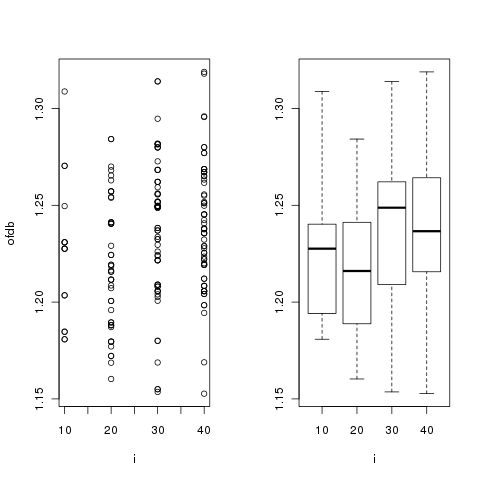
\includegraphics[width=0.5\textwidth]{./figures/ga_i.png}}
  \subfloat[$f \sim tt$]{\label{fig:ga_tt}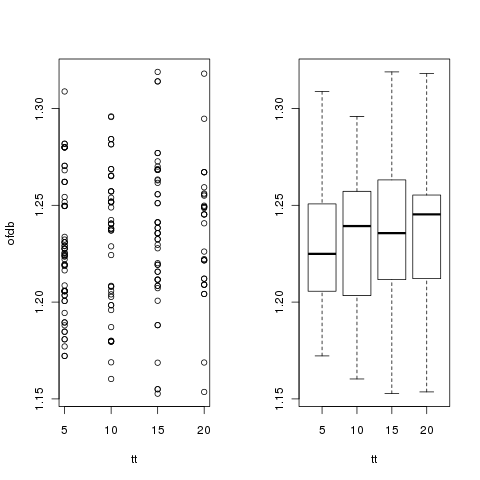
\includegraphics[width=0.5\textwidth]{./figures/ga_tt.png}}
  \label{fig:f_ga1}
\end{figure}

\begin{figure}[H]
  \centering
  \subfloat[$f \sim pc$]{\label{fig:ga_pc}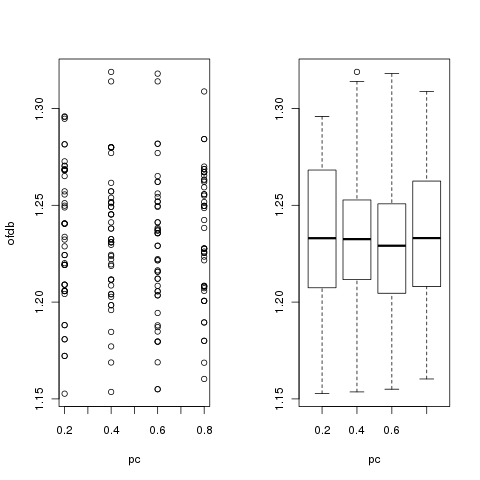
\includegraphics[width=0.5\textwidth]{./figures/ga_pc.png}}
  \subfloat[$f \sim pm$]{\label{fig:ga_pm}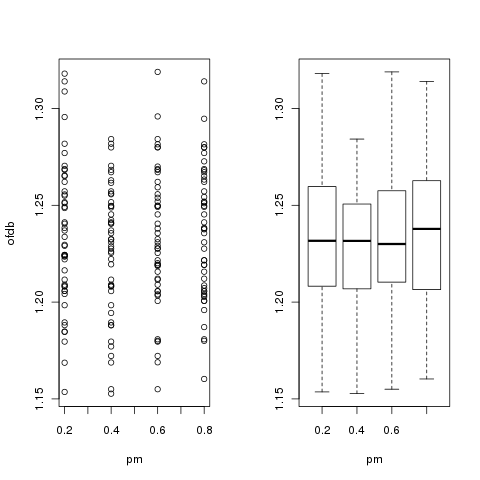
\includegraphics[width=0.5\textwidth]{./figures/ga_pm.png}}
  \label{fig:f_ga2}
\end{figure}

    Se puede concluir de las gráficas:
\begin{itemize}
    \item Para todos los parámetros, no se puede observar una
relación lineal con respecto a $f$.
\end{itemize}

\subsubsection{\emph{GAH} para datos numéricos}

    Los resultados para datos númericos se presentan a continuación:

\begin{figure}[H]
  \centering
  \subfloat[$f \sim I$]{\label{fig:ga_csv_i}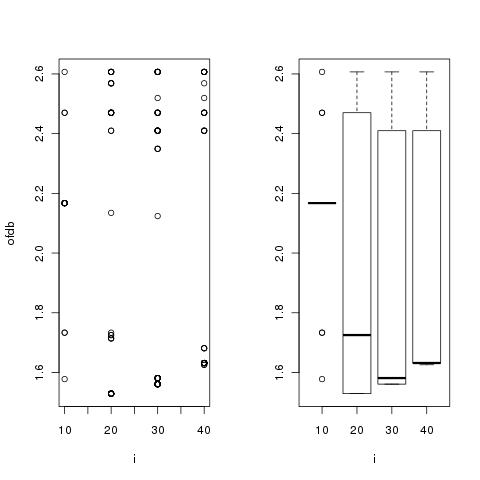
\includegraphics[width=0.5\textwidth]{./figures/ga_csv_i.png}}
  \subfloat[$f \sim tt$]{\label{fig:ga_csv_tt}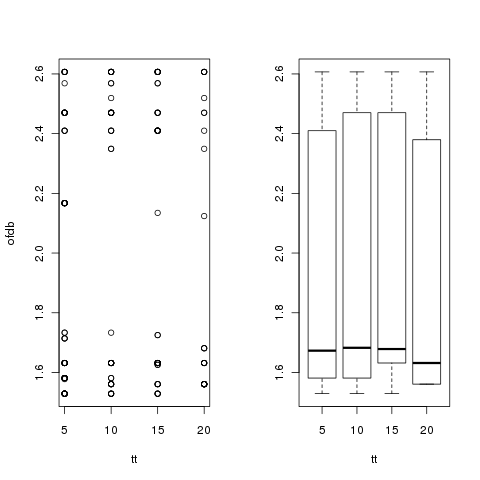
\includegraphics[width=0.5\textwidth]{./figures/ga_csv_tt.png}}
  \label{fig:f_gacsv1}
\end{figure}

\begin{figure}[H]
  \centering
  \subfloat[$f \sim pc$]{\label{fig:ga_csv_pc}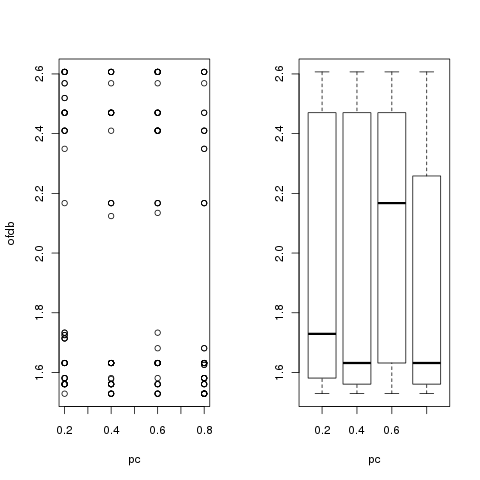
\includegraphics[width=0.5\textwidth]{./figures/ga_csv_pc.png}}
  \subfloat[$f \sim pm$]{\label{fig:ga_csv_pm}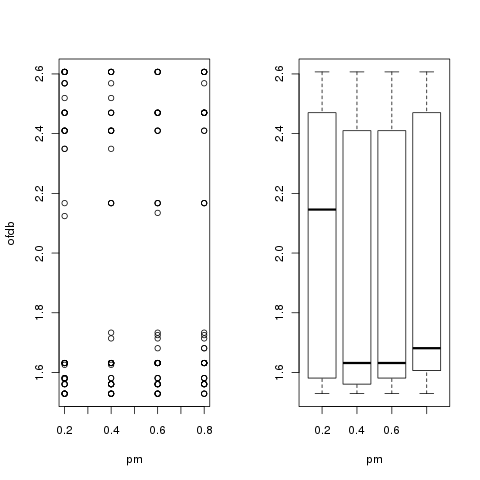
\includegraphics[width=0.5\textwidth]{./figures/ga_csv_pm.png}}
  \label{fig:f_gacsv2}
\end{figure}

	Se puede concluir de las gráficas:
\begin{itemize}
	\item De forma similar a las imágenes, ningún parámetro tiene
un comportamiento lineal con respecto a $f$.
\end{itemize}

\subsection{Algoritmo \emph{NPSOH}}\label{sect:inpso-rv}

    Las variables del \emph{NPSOH}(\ref{sect:inpso}) son las siguientes:
\begin{itemize}
    \item $I$: tamaño de la población. Se varió su valor en el rango
$[10, 20, \cdots, 40]$.
    \item $c_1$: factor de la componente cognitiva. Se varió su valor en el
rango $[0.5; 1.0; \cdots; 2.0]$
    \item $c_2$: factor de la componente social. Se varió en el rango
$[0.5; 1.0; \cdots; 2.0]$
    \item $W$: peso inercial de la partícula. Se varió su valor en el rango
$[0.6; 0.8; \cdots; 1.2]$.
    \item $vmx$: velocidad máxima de la partícula. Se varió su valor en el rango
$[0.1; 0.4; \cdots; 1.0]$.
\end{itemize}

\subsubsection{\emph{NPSOH} para imágenes}

	A continuación, se presentan las gráficas de cada uno de los
parámetros en relación con la variable $f$ cuando los datos del algoritmo
pertenecen a imágenes:

\begin{figure}[H]
  \centering
  \subfloat[$f \sim I$]{\label{fig:pso_i}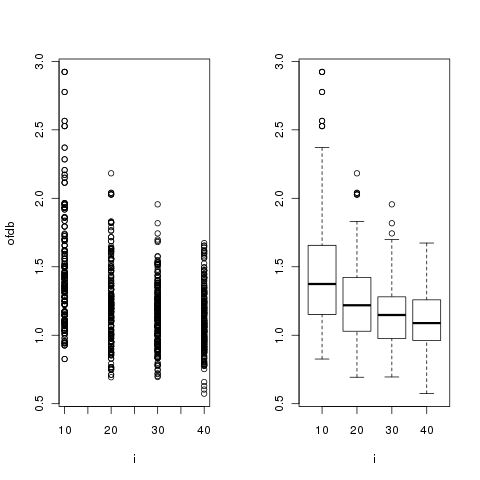
\includegraphics[width=0.5\textwidth]{./figures/pso_i.png}}
  \subfloat[$f \sim c_1$]{\label{fig:pso_c1}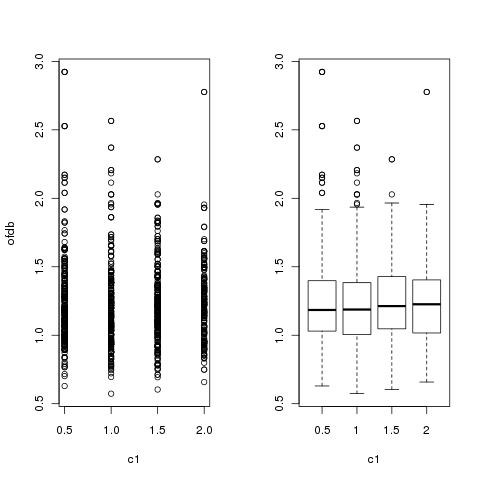
\includegraphics[width=0.5\textwidth]{./figures/pso_c1.png}}
  \label{fig:f_pso1}
\end{figure}

\begin{figure}[H]
  \centering
  \subfloat[$f \sim c_2$]{\label{fig:pso_c2}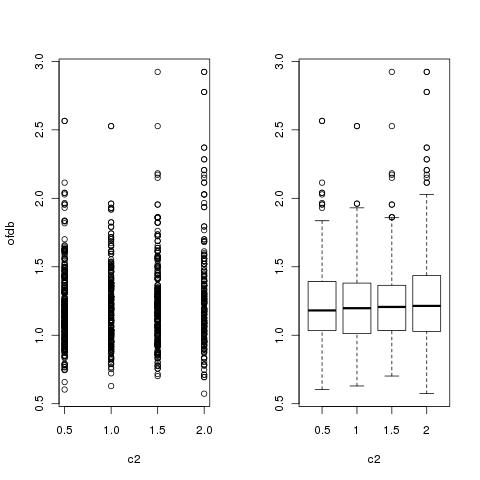
\includegraphics[width=0.5\textwidth]{./figures/pso_c2.png}}
  \subfloat[$f \sim W$]{\label{fig:pso_w}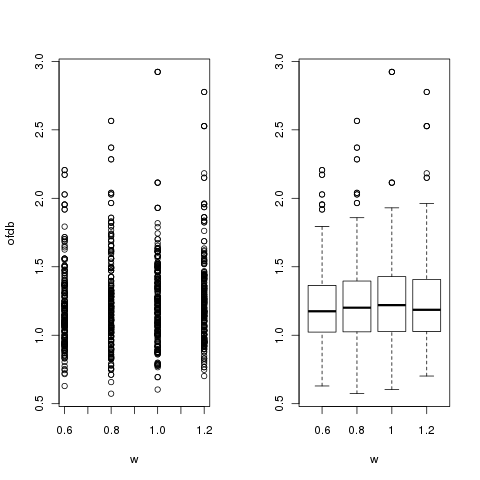
\includegraphics[width=0.5\textwidth]{./figures/pso_w.png}}
  \label{fig:f_pso2}
\end{figure}

\begin{figure}[H]
  \centering
  \subfloat[$f \sim vmx$]{\label{fig:pso_vmx}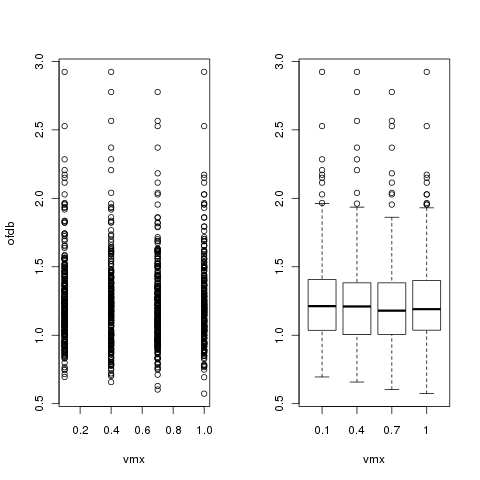
\includegraphics[width=0.5\textwidth]{./figures/pso_vmx.png}}
  \label{fig:f_pso3}
\end{figure}

    Se puede concluir de las gráficas:
\begin{itemize}
    \item Para el parámetro $I$, se puede observar cierto escalonamiento,
pero, aún así, las cajas se solapan. Es probable que no exista una
relación lineal entre este parámetro y $f$.
    \item Para los parámetros $c_1$, $c_2$, $W$ y $vmx$, se puede
observar una relación constante y con cajas solapadas. Es probable
que no exista una relación lineal entre estos parámetros y $f$.
\end{itemize}

\subsubsection{\emph{NPSOH} para datos numéricos}

    Los resultados para datos númericos se presentan a continuación:

\begin{figure}[H]
  \centering
  \subfloat[$f \sim I$]{\label{fig:pso_csv_i}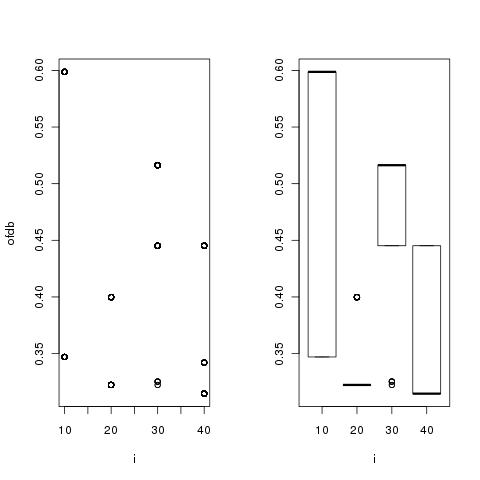
\includegraphics[width=0.5\textwidth]{./figures/pso_csv_i.png}}
  \subfloat[$f \sim c_1$]{\label{fig:pso_csv_c1}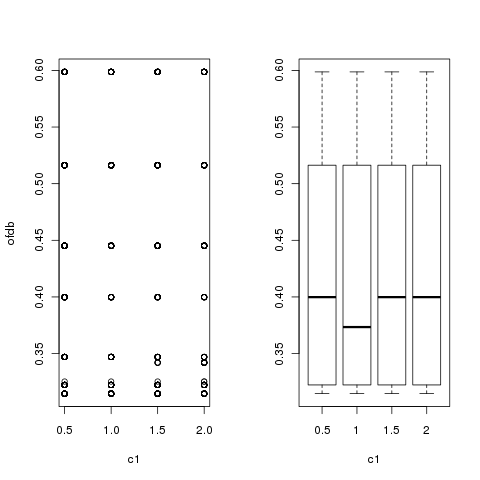
\includegraphics[width=0.5\textwidth]{./figures/pso_csv_c1.png}}
  \label{fig:f_pso_csv1}
\end{figure}

\begin{figure}[H]
  \centering
  \subfloat[$f \sim c_2$]{\label{fig:pso_csv_c2}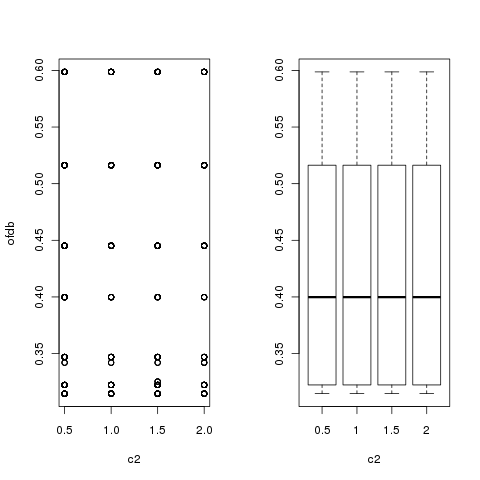
\includegraphics[width=0.5\textwidth]{./figures/pso_csv_c2.png}}
  \subfloat[$f \sim W$]{\label{fig:pso_csv_w}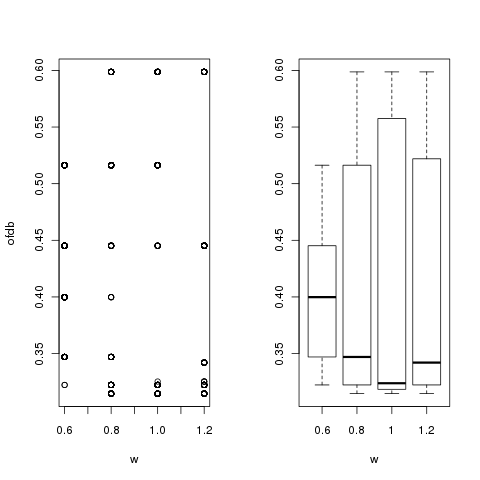
\includegraphics[width=0.5\textwidth]{./figures/pso_csv_w.png}}
  \label{fig:f_pso_csv2}
\end{figure}

\begin{figure}[H]
  \centering
  \subfloat[$f \sim vmx$]{\label{fig:pso_csv_vmx}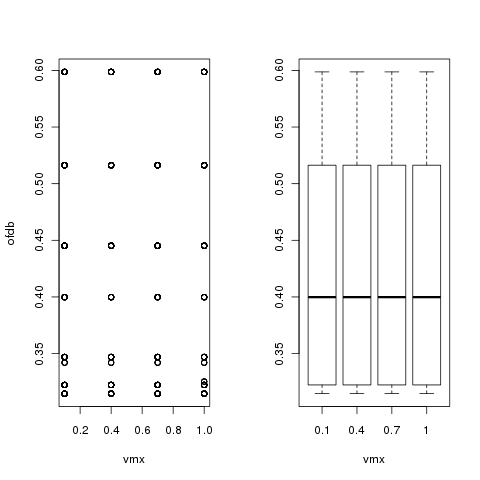
\includegraphics[width=0.5\textwidth]{./figures/pso_csv_vmx.png}}
  \label{fig:f_pso_csv3}
\end{figure}

	Se puede concluir de las gráficas:
\begin{itemize}
	\item Para datos numéricos con más de tres dimensiones, ninguno de los
parámetros del \emph{NPSOH} conserva una relación de linealidad con la variable
aleatoria dependiente $f$.
\end{itemize}

\subsection{Algoritmo \emph{WPSOH}}\label{sect:iwpso-rv}

    Las variables del \emph{WPSOH}(\ref{sect:iwpso}) son las siguientes:
\begin{itemize}
    \item $I$: tamaño de la población. Se varió su valor en el rango
$[10, 20, \cdots, 40]$.
    \item $c_1$: factor de la componente cognitiva. Se varió su valor en el
rango $[0.5; 1.0; \cdots; 2.0]$
    \item $c_2$: factor de la componente social. Se varió en el rango
$[0.5; 1.0; \cdots; 2.0]$
    \item $W$: peso inercial de la partícula. Se varió su valor en el rango
$[0.6; 0.8; \cdots; 1.2]$.
    \item $vmx$: velocidad máxima de la partícula. Se varió su valor en el rango
$[0.1; 0.4; \cdots; 1.0]$.
	\item $w_1$: peso de la distancia promedio entre elementos de un
mismo cluster (distancia intra-cluster promedio). Se varió su valor en el rango
$[0.0; 0.5; 1.0]$
	\item $w_2$: peso de la distancia promedio entre los diferentes
clusters (distancia inter-cluster promedio). Se varió su valor en el rango
$[0.0; 0.5; 1.0]$
	\item $w_3$: peso de el error. Se varió su valor en el rango
$[0.0; 0.5; 1.0]$
\end{itemize}

\subsubsection{\emph{WPSOH} para imágenes}

	A continuación, se presentan las gráficas de cada uno de los
parámetros en relación con la variable $f$ cuando los datos
del algoritmo pertenecen a imágenes:

\begin{figure}[H]
  \centering
  \subfloat[$f \sim I$]{\label{fig:wpso_i}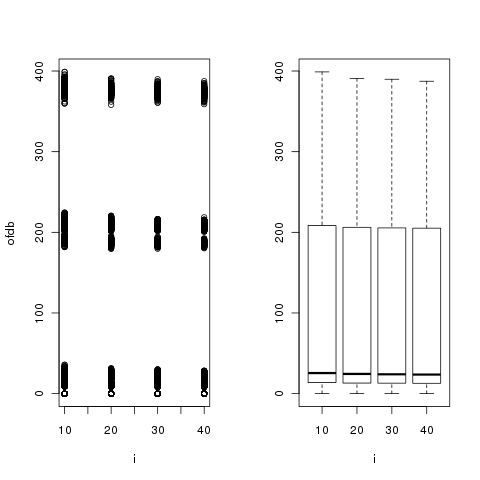
\includegraphics[width=0.5\textwidth]{./figures/wpso_i.png}}
  \subfloat[$f \sim c_1$]{\label{fig:wpso_c1}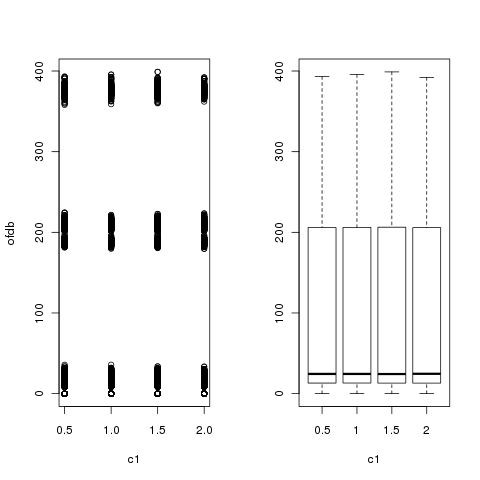
\includegraphics[width=0.5\textwidth]{./figures/wpso_c1.png}}
  \label{fig:f_wpso1}
\end{figure}

\begin{figure}[H]
  \centering
  \subfloat[$f \sim c_2$]{\label{fig:wpso_c2}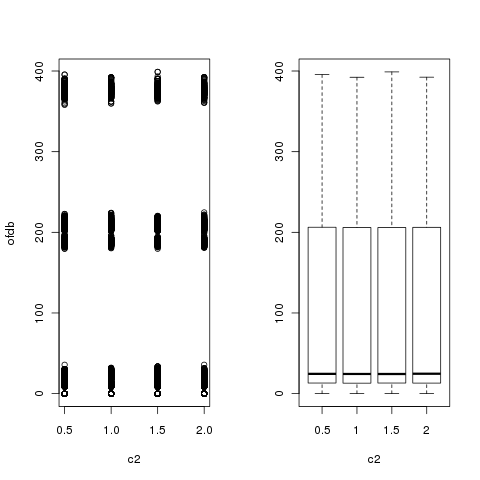
\includegraphics[width=0.5\textwidth]{./figures/wpso_c2.png}}
  \subfloat[$f \sim W$]{\label{fig:wpso_w}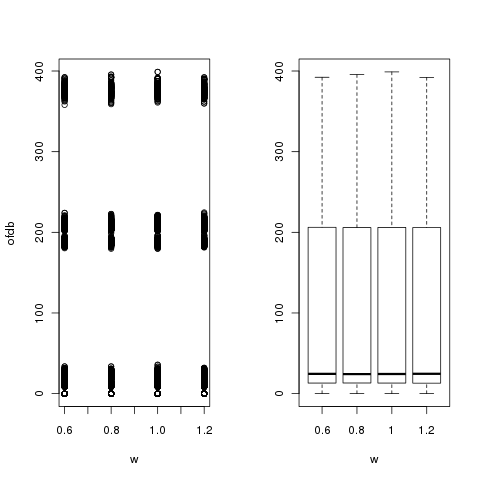
\includegraphics[width=0.5\textwidth]{./figures/wpso_w.png}}
  \label{fig:f_wpso2}
\end{figure}

\begin{figure}[H]
  \centering
  \subfloat[$f \sim vmx$]{\label{fig:wpso_vmx}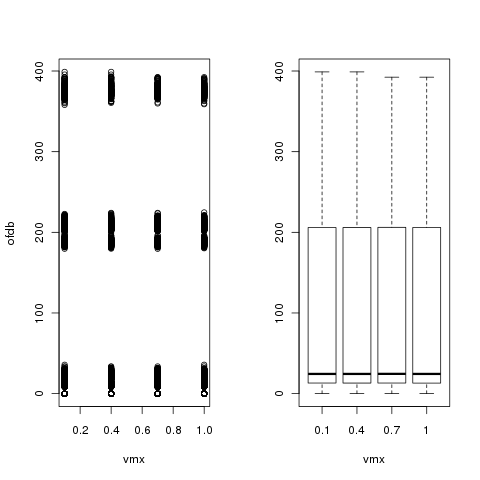
\includegraphics[width=0.5\textwidth]{./figures/wpso_vmx.png}}
  \subfloat[$f \sim w_1$]{\label{fig:wpso_w1}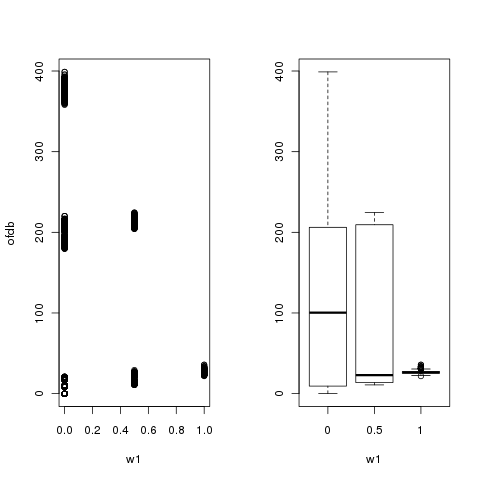
\includegraphics[width=0.5\textwidth]{./figures/wpso_w1.png}}
  \label{fig:f_wpso3}
\end{figure}

\begin{figure}[H]
  \centering
  \subfloat[$f \sim w_2$]{\label{fig:wpso_w2}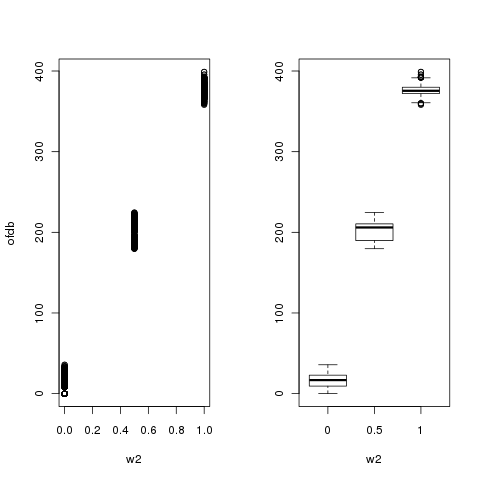
\includegraphics[width=0.5\textwidth]{./figures/wpso_w2.png}}
  \subfloat[$f \sim w_3$]{\label{fig:wpso_w3}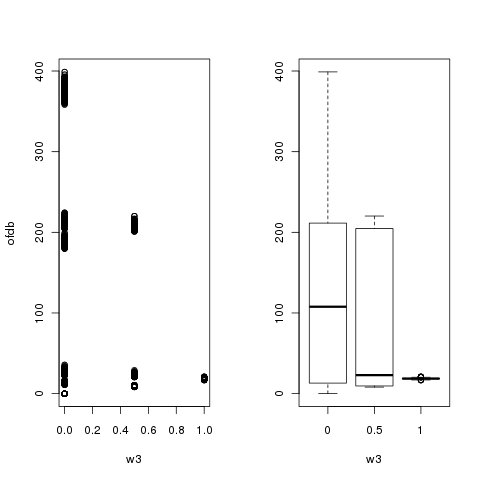
\includegraphics[width=0.5\textwidth]{./figures/wpso_w3.png}}
  \label{fig:f_wpso4}
\end{figure}

    Se puede concluir de las gráficas:
\begin{itemize}
    \item Para el parámetro $w_2$, es probable que exista una
relación lineal con la variable $f$.
    \item Para los demás parámetros no se observan relaciones
lineales ya que no hay escalonamiento.
\end{itemize}

\subsubsection{\emph{WPSOH} para datos numéricos}

    Los resultados para datos númericos se presentan a continuación:

\begin{figure}[H]
  \centering
  \subfloat[$f \sim I$]{\label{fig:wpso_csv_i}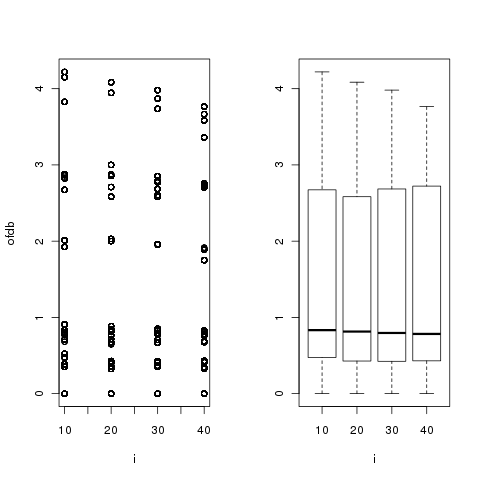
\includegraphics[width=0.5\textwidth]{./figures/wpso_csv_i.png}}
  \subfloat[$f \sim c_1$]{\label{fig:wpso_csv_c1}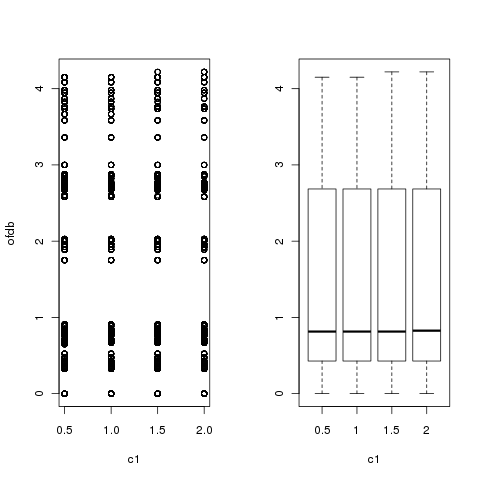
\includegraphics[width=0.5\textwidth]{./figures/wpso_csv_c1.png}}
  \label{fig:f_wpso_csv1}
\end{figure}

\begin{figure}[H]
  \centering
  \subfloat[$f \sim c_2$]{\label{fig:wpso_csv_c2}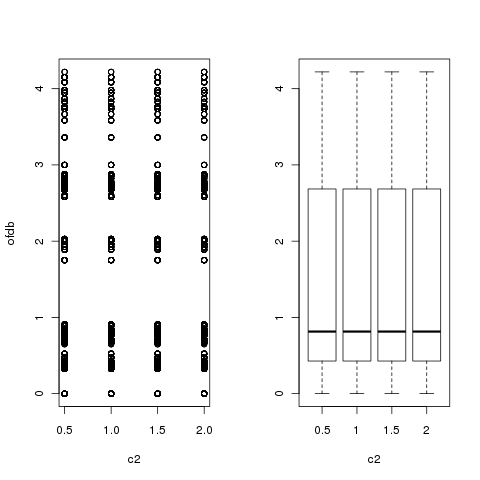
\includegraphics[width=0.5\textwidth]{./figures/wpso_csv_c2.png}}
  \subfloat[$f \sim W$]{\label{fig:wpso_csv_w}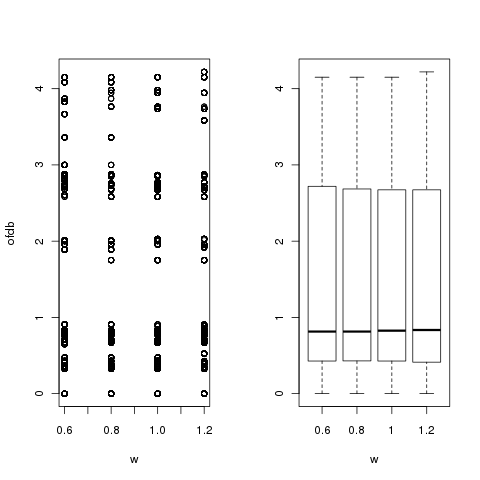
\includegraphics[width=0.5\textwidth]{./figures/wpso_csv_w.png}}
  \label{fig:f_wpso_csv2}
\end{figure}

\begin{figure}[H]
  \centering
  \subfloat[$f \sim vmx$]{\label{fig:wpso_csv_vmx}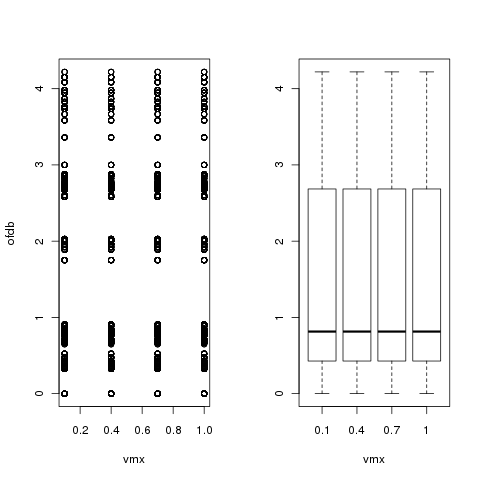
\includegraphics[width=0.5\textwidth]{./figures/wpso_csv_vmx.png}}
  \subfloat[$f \sim w_1$]{\label{fig:wpso_csv_w1}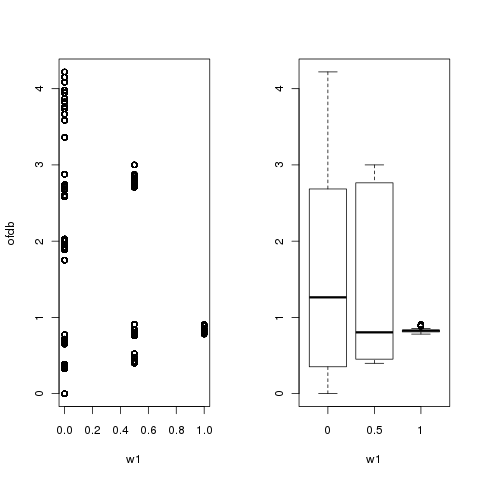
\includegraphics[width=0.5\textwidth]{./figures/wpso_csv_w1.png}}
  \label{fig:f_wpso_csv3}
\end{figure}

\begin{figure}[H]
  \centering
  \subfloat[$f \sim w_2$]{\label{fig:wpso_csv_w2}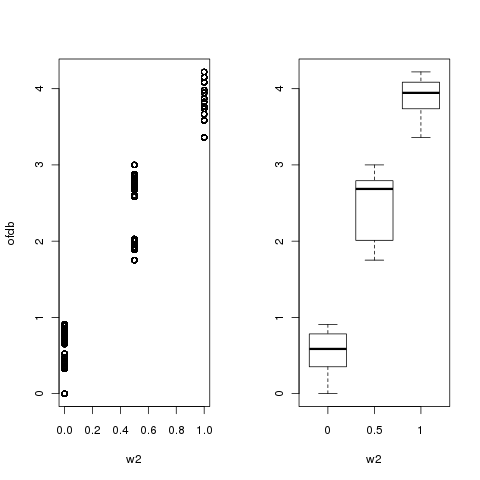
\includegraphics[width=0.5\textwidth]{./figures/wpso_csv_w2.png}}
  \subfloat[$f \sim w_3$]{\label{fig:wpso_csv_w3}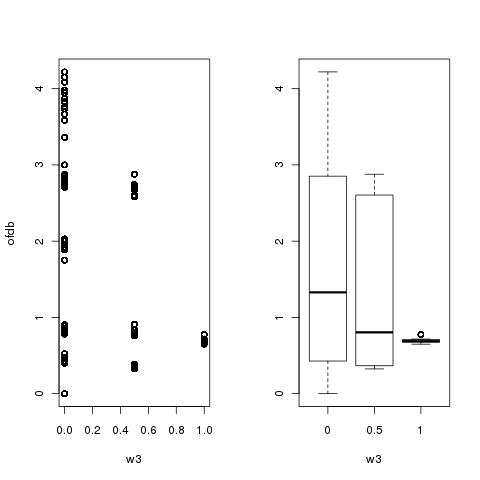
\includegraphics[width=0.5\textwidth]{./figures/wpso_csv_w3.png}}
  \label{fig:f_wpso_csv4}
\end{figure}

	Se puede concluir de las gráficas:
\begin{itemize}
	\item De forma similar a las imágenes, el único parámetro con
un comportamiento lineal con respecto a $f$ es $w_2$.
\end{itemize}

\subsection{Algoritmo \emph{NDEH}}\label{sect:inde-rv}

    Las variables del \emph{NDEH}(\ref{sect:ide}) son las siguientes:
\begin{itemize}
    \item $I$: tamaño de la población. Se varió su valor en el rango
$[10, 20, \cdots, 40]$.
    \item $w_1$: peso de la distancia intracluster. Se varió en el rango
$[0.0; 0.5; 1.0]$.
    \item $w_2$: peso de distancia intercluster. Se varió en el rango
$[0.0; 0.5; 1.0]$.
    \item $w_3$: peso del error. Se varió en el rango
$[0.0; 0.5; 1.0]$.
\end{itemize}

\subsubsection{\emph{NDEH} para imágenes}

	A continuación, se presentan las gráficas de cada uno de los
parámetros en relación con la variable $f$ cuando los datos
del algoritmo pertenecen a imágenes:

\begin{figure}[H]
  \centering
  \subfloat[$f \sim I$]{\label{fig:de_i}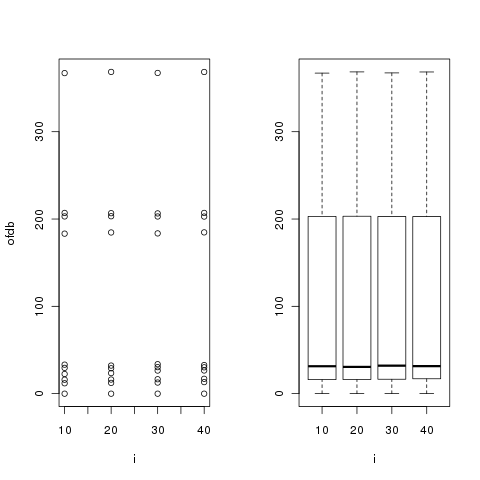
\includegraphics[width=0.5\textwidth]{./figures/de_i.png}}
  \subfloat[$f \sim w_1$]{\label{fig:de_w1}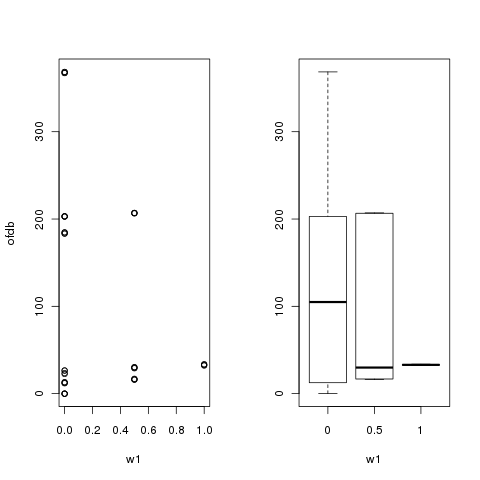
\includegraphics[width=0.5\textwidth]{./figures/de_w1.png}}
  \label{fig:f_de1}
\end{figure}

\begin{figure}[H]
  \centering
  \subfloat[$f \sim w_2$]{\label{fig:de_w2}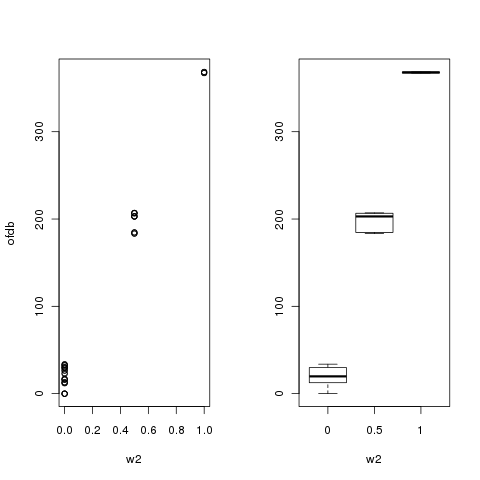
\includegraphics[width=0.5\textwidth]{./figures/de_w2.png}}
  \subfloat[$f \sim w_3$]{\label{fig:de_w3}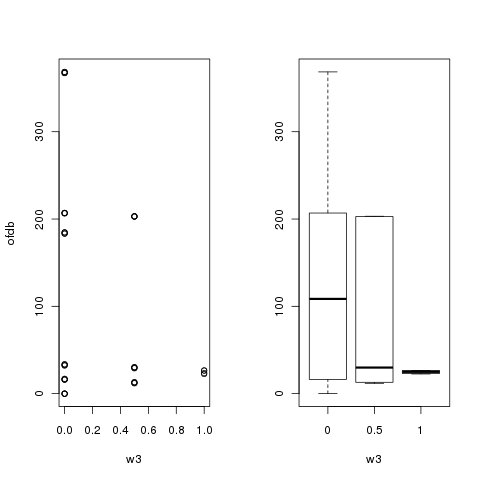
\includegraphics[width=0.5\textwidth]{./figures/de_w3.png}}
  \label{fig:f_de1}
\end{figure}

    Se puede concluir de las gráficas:
\begin{itemize}
    \item Para el parámetro $w_2$, es probable que exista una
relación lineal con la variable $f$.
    \item Para los demás parámetros no se observan relaciones
lineales ya que no hay escalonamiento.
\end{itemize}

\subsubsection{\emph{NDEH} para datos numéricos}

    Los resultados para datos númericos se presentan a continuación:

\begin{figure}[H]
  \centering
  \subfloat[$f\sim I$]{\label{fig:de_csv_i}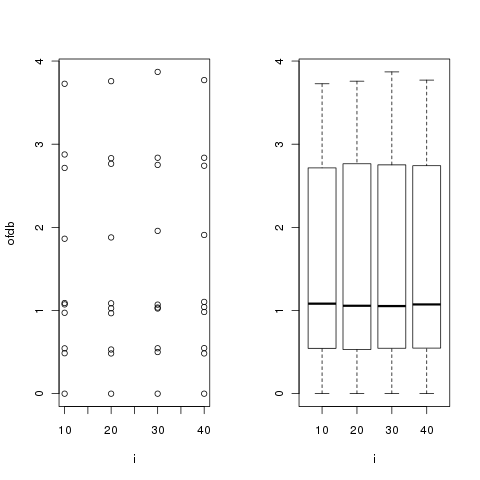
\includegraphics[width=0.5\textwidth]{./figures/de_csv_i.png}}
  \subfloat[$f \sim w_1$]{\label{fig:de_csv_w1}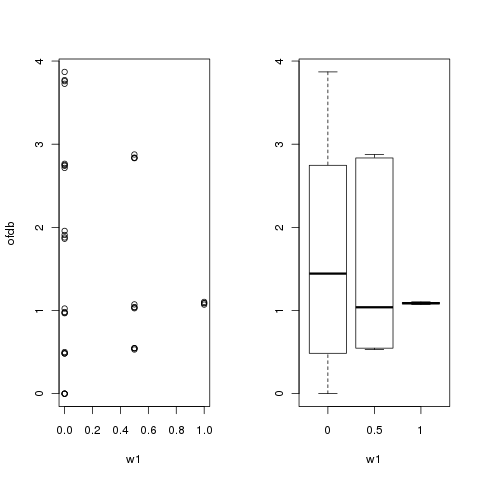
\includegraphics[width=0.5\textwidth]{./figures/de_csv_w1.png}}
  \label{fig:f_de_csv1}
\end{figure}

\begin{figure}[H]
  \centering
  \subfloat[$f \sim w_2$]{\label{fig:de_csv_w2}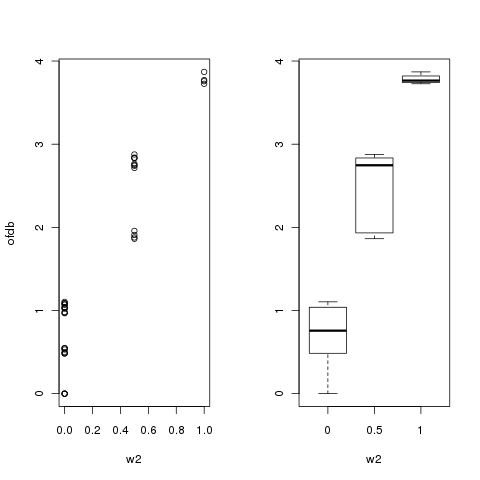
\includegraphics[width=0.5\textwidth]{./figures/de_csv_w2.png}}
  \subfloat[$f \sim w_3$]{\label{fig:de_csv_w3}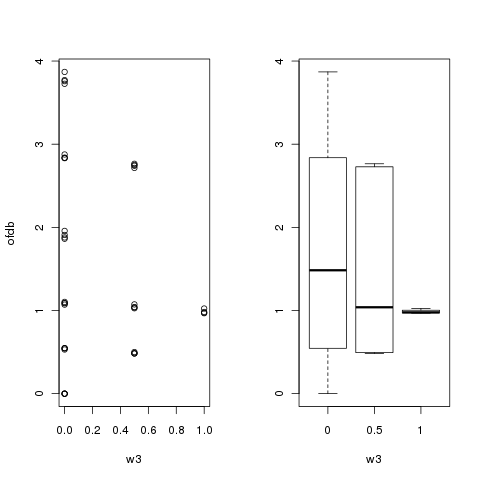
\includegraphics[width=0.5\textwidth]{./figures/de_csv_w3.png}}
  \label{fig:f_de_csv1}
\end{figure}

	Se puede concluir de las gráficas:
\begin{itemize}
	\item De forma similar a las imágenes, el único parámetro con
un comportamiento lineal con respecto a $f$ es $w_2$.
\end{itemize}

\subsection{Algoritmo \emph{SDEH}}\label{sect:isde-rv}

    Las variables del \emph{SDEH}(\ref{sect:ide}) son las siguientes:
\begin{itemize}
    \item $I$: tamaño de la población. Se varió su valor en el rango
$[10, 20, \cdots, 40]$.
    \item $w_1$: peso de la distancia intracluster. Se varió en el rango
$[0.0; 0.5; 1.0]$.
    \item $w_2$: peso de distancia intercluster. Se varió en el rango
$[0.0; 0.5; 1.0]$.
    \item $w_3$: peso del error. Se varió en el rango
$[0.0; 0.5; 1.0]$.
	\item $\gamma$: valor de escalamiento de los vectores. Se varió en el rango
$[0.1; 0.3; \cdots; 0.9]$.
	\item $Cr$: probabilidad de cruce. Se varió en el rango
$[0.1; 0.3; \cdots; 0.9]$.
\end{itemize}

\subsubsection{\emph{SDEH} para imágenes}

	A continuación, se presentan las gráficas de cada uno de los
parámetros en relación con la variable $f$ cuando los datos
del algoritmo pertenecen a imágenes:

\begin{figure}[H]
  \centering
  \subfloat[$f \sim I$]{\label{fig:sde_i}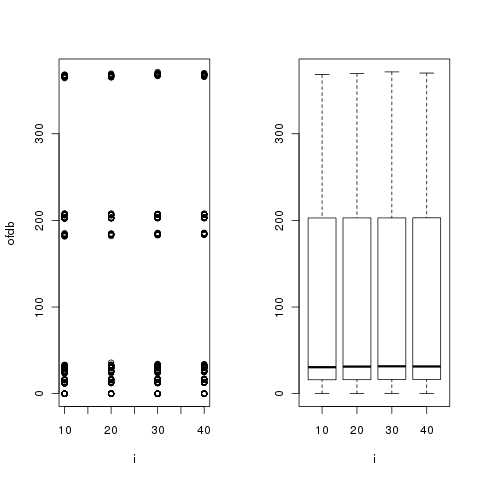
\includegraphics[width=0.5\textwidth]{./figures/sde_i.png}}
  \subfloat[$f \sim w_1$]{\label{fig:sde_w1}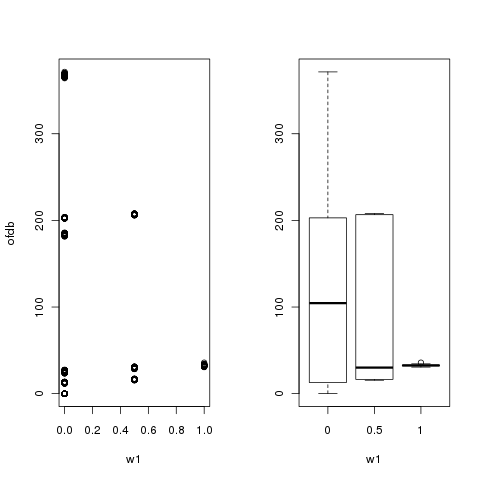
\includegraphics[width=0.5\textwidth]{./figures/sde_w1.png}}
  \label{fig:f_sde1}
\end{figure}

\begin{figure}[H]
  \centering
  \subfloat[$f \sim w_2$]{\label{fig:sde_w2}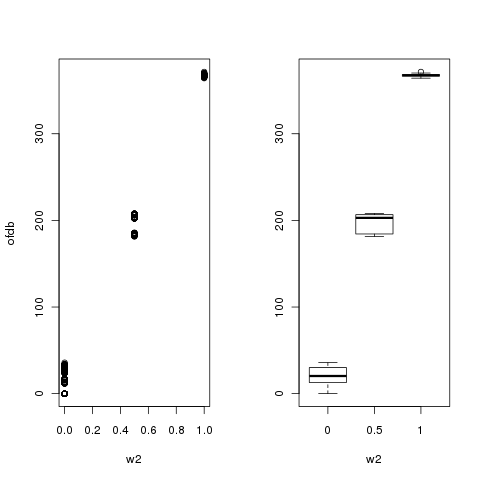
\includegraphics[width=0.5\textwidth]{./figures/sde_w2.png}}
  \subfloat[$f \sim w_3$]{\label{fig:sde_w3}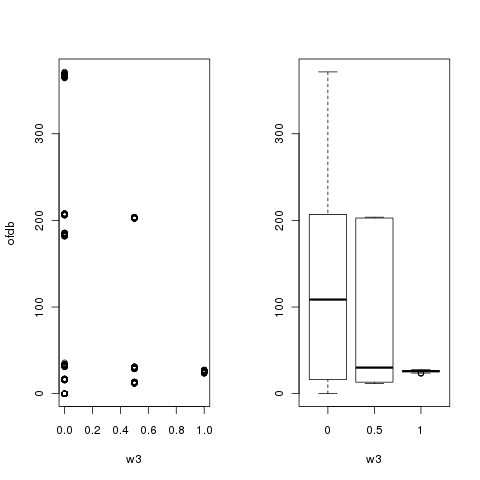
\includegraphics[width=0.5\textwidth]{./figures/sde_w3.png}}
  \label{fig:f_sde2}
\end{figure}

\begin{figure}[H]
  \centering
  \subfloat[$f \sim \gamma$]{\label{fig:sde_f}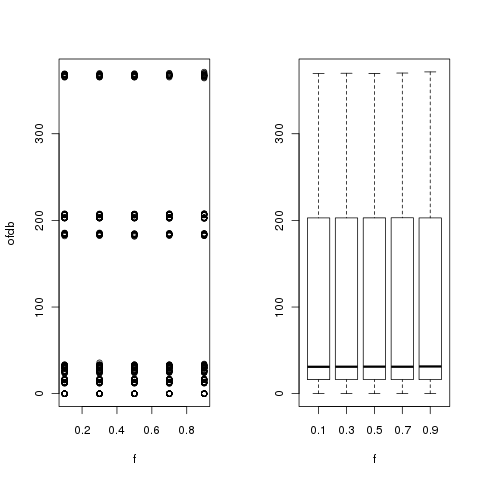
\includegraphics[width=0.5\textwidth]{./figures/sde_f.png}}
  \subfloat[$f \sim Cr$]{\label{fig:sde_pc}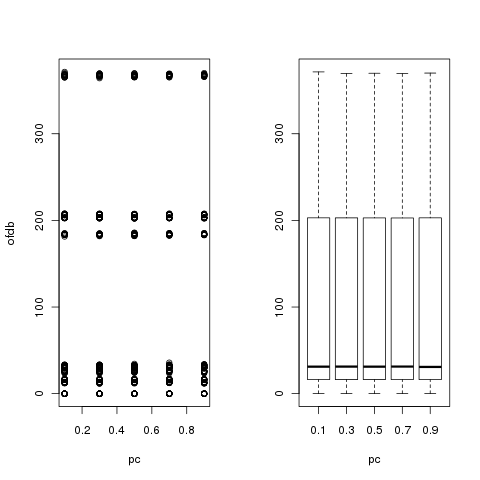
\includegraphics[width=0.5\textwidth]{./figures/sde_pc.png}}
  \label{fig:f_sde3}
\end{figure}

    Se puede concluir de las gráficas:
\begin{itemize}
    \item Para el parámetro $w_2$, es probable que exista una
relación lineal con la variable $f$.
    \item Para los demás parámetros no se observan relaciones
lineales ya que no hay escalonamiento.
\end{itemize}

\subsubsection{\emph{SDEH} para datos numéricos}

    Los resultados para datos númericos se presentan a continuación:

\begin{figure}[H]
  \centering
  \subfloat[$f \sim I$]{\label{fig:sde_csv_i}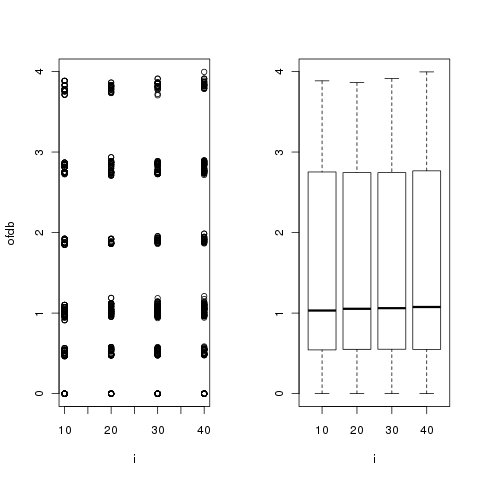
\includegraphics[width=0.5\textwidth]{./figures/sde_csv_i.png}}
  \subfloat[$f \sim w_1$]{\label{fig:sde_csv_w1}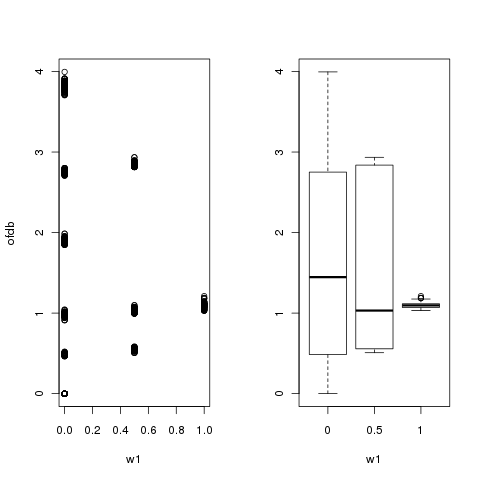
\includegraphics[width=0.5\textwidth]{./figures/sde_csv_w1.png}}
  \label{fig:f_sde_csv1}
\end{figure}

\begin{figure}[H]
  \centering
  \subfloat[$f \sim w_2$]{\label{fig:sde_csv_w2}\includegraphics[width=0.5\textwidth]{./figures/sde_csv_w2.png}}
  \subfloat[$f \sim w_3$]{\label{fig:sde_csv_w3}\includegraphics[width=0.5\textwidth]{./figures/sde_csv_w3.png}}
  \label{fig:f_sde_csv2}
\end{figure}

\begin{figure}[H]
  \centering
  \subfloat[$f \sim \gamma$]{\label{fig:sde_csv_f}\includegraphics[width=0.5\textwidth]{./figures/sde_csv_f.png}}
  \subfloat[$f \sim Cr$]{\label{fig:sde_csv_pc}\includegraphics[width=0.5\textwidth]{./figures/sde_csv_pc.png}}
  \label{fig:f_sde_csv3}
\end{figure}

	Se puede concluir de las gráficas:
\begin{itemize}
	\item De forma similar a las imágenes, el único parámetro con
un comportamiento lineal con respecto a $f$ es $w_2$.
\end{itemize}

\subsection{Algoritmo de Abeja (\emph{BeeH})}\label{sect:ibee-rv}

    Las variables del \emph{BeeH} (\ref{sect:ibee}) son las siguientes:
\begin{itemize}
    \item $I$: cantidad de abejas. Se varió su valor en el rango
$[5, 10, \cdots, 40]$.
    \item $m$: cantidad de lugares de flores. Se varió su valor en el rango
$[4, 6, \cdots, 10]$.
    \item $e$: cantidad de sitios élite de flores. Se varió su valor en el rango
$[1, 3, \cdots, 10]$.
    \item $eb$: cantidad de abejas élite. Se varió su valor en el rango
$[4, 6, \cdots, 10]$.
	\item $ob$: cantidad de abejas exploradoras. Se varió su valor en el rango
$[1, 3, \cdots, 10]$.
\end{itemize}

\subsubsection{\emph{BeeH} para imágenes}

	A continuación, se presentan las gráficas de cada uno de los
parámetros en relación con la variable $f$ cuando los datos
del algoritmo pertenecen a imágenes:

\begin{figure}[H]
  \centering
  \subfloat[$f \sim I$]{\label{fig:bee_i}\includegraphics[width=0.5\textwidth]{./figures/bee_i.png}}
  \subfloat[$f \sim m$]{\label{fig:bee_m}\includegraphics[width=0.5\textwidth]{./figures/bee_m.png}}
  \label{fig:f_bee1}
\end{figure}

\begin{figure}[H]
  \centering
  \subfloat[$f \sim e$]{\label{fig:bee_e}\includegraphics[width=0.5\textwidth]{./figures/bee_e.png}}
  \subfloat[$f \sim eb$]{\label{fig:bee_eb}\includegraphics[width=0.5\textwidth]{./figures/bee_eb.png}}
  \label{fig:f_bee2}
\end{figure}

\begin{figure}[H]
  \centering
  \subfloat[$f \sim ob$]{\label{fig:bee_ob}\includegraphics[width=0.5\textwidth]{./figures/bee_ob.png}}
  \label{fig:f_bee3}
\end{figure}

    Se puede concluir de las gráficas:
\begin{itemize}
	\item Aunque parámetros como $e$, $eb$ y $ob$ tienen cierta
linealidad con respecto a $f$, las cajas se solapan, por lo tanto
es probable que no exista una relación de linealidad entre estos
y $f$.
	\item Los demás parámetros tiene una relación constante con
$f$.
\end{itemize}

\subsubsection{\emph{BeeH} para datos numéricos}

    Los resultados para datos númericos se presentan a continuación:

\begin{figure}[H]
  \centering
  \subfloat[$f \sim I$]{\label{fig:bee_csv_i}\includegraphics[width=0.5\textwidth]{./figures/bee_csv_i.png}}
  \subfloat[$f \sim m$]{\label{fig:bee_csv_m}\includegraphics[width=0.5\textwidth]{./figures/bee_csv_m.png}}
  \label{fig:f_bee1}
\end{figure}

\begin{figure}[H]
  \centering
  \subfloat[$f \sim e$]{\label{fig:bee_csv_e}\includegraphics[width=0.5\textwidth]{./figures/bee_csv_e.png}}
  \subfloat[$f \sim eb$]{\label{fig:bee_csv_eb}\includegraphics[width=0.5\textwidth]{./figures/bee_csv_eb.png}}
  \label{fig:f_bee2}
\end{figure}

\begin{figure}[H]
  \centering
  \subfloat[$f \sim ob$]{\label{fig:bee_csv_ob}\includegraphics[width=0.5\textwidth]{./figures/bee_csv_ob.png}}
  \label{fig:f_bee3}
\end{figure}

    Se puede concluir de las gráficas:
\begin{itemize}
	\item Aunque el parámetro como $i$ tiene cierta linealidad con
respecto a $f$, las cajas se solapan, por lo tanto es probable
que no exista una relación de linealidad entre éste y $f$.
	\item Los demás parámetros tiene una relación constante con
$f$.
\end{itemize}

\subsection{Algoritmo de Hormiga (\emph{AntH})}\label{sect:iant-rv}

    La variable del \emph{AntH} (\ref{sect:ihormiga}) es la siguiente:
\begin{itemize}
    \item $I$: tamaño de la población. Se varió su valor en el rango
$[5, 10, \cdots, 40]$.
\end{itemize}

\subsubsection{\emph{AntH} para imágenes}

	A continuación, se presentan las gráficas de cada uno de los
parámetros en relación con la variable $f$ cuando los datos
del algoritmo pertenecen a imágenes:

\begin{figure}[H]
  \centering
  \subfloat[$f \sim I$]{\label{fig:ant_i}\includegraphics[width=0.5\textwidth]{./figures/ant_i.png}}
  \label{fig:f_ant}
\end{figure}

    Se puede concluir de las gráficas:
\begin{itemize}
    \item Para el parámetro $I$, se puede observar que las cajas están solapadas
y no tiene forma escalonada, así que es probable que no exista
una relación de linealidad con $f$.
\end{itemize}

\subsubsection{\emph{AntH} para datos numéricos}

    Los resultados para datos númericos se presentan a continuación:

\begin{figure}[H]
  \centering
  \subfloat[f~I]{\label{fig:ant_csv_i}\includegraphics[width=0.5\textwidth]{./figures/ant_csv_i.png}}
  \label{fig:f_ant}
\end{figure}

    Se puede concluir de las gráficas:
\begin{itemize}
	\item De forma similar a las imágenes, $I$ no tiene un
comportamiento lineal con respecto a $f$.
\end{itemize}


\section{Análisis numérico}

    En esta sección, se presenta un resumen de las pruebas de linealidad de
los parámetros de las diferentes metaheurísticas y la función de \emph{fitness}
$f$ de sus soluciones finales.

\subsection{Correlación}

    Para que tenga sentido suponer linealidad de una variable $X$
con respecto a $Y$, se necesita que la correlación entre ellas esté
cercana a 1. Para esto se hace una prueba de hipótesis para $\rho(Y, X)$ donde:
\begin{itemize}
    \item $H_0$: $\rho(Y, X) = \rho_0$.
    \item $H_1$: $\rho(Y, X) \neq \rho_0$. La relación es lineal.
\end{itemize}
para
\begin{itemize}
    \item $\rho_0 = 0$.
    \item $Y$ es una variable aleatoria dependiente que debería estar
en función de $X$. $X$ es una variable aleatoria independiente y $n$
es el tamaño de la muestra. Se define entonces el modelo estadístico
lineal de la siguiente forma:
        \begin{center}
            $Y = \hat{\beta_0} + \hat{\beta_1} \cdot X$
        \end{center}
\end{itemize}

    El estimador de máxima verosimilitud de $\rho(Y, X)$ está
dado por el coeficiente de correlación muestral \cite{AB_0}:
\begin{center}
    $r = \hat{\beta_1}\displaystyle\sqrt{\frac{S_{xx}}{S_{yy}}}$
\end{center}
donde:
\begin{itemize}
    \item $S_{xx} = \displaystyle\sum_{i = 1}^n (X_i - \bar{X})^2$
    \item $S_{xy} = \displaystyle\sum_{i = 1}^n (X_i - \bar{X}) \cdot (Y_i - \bar{Y})$
    \item $\hat{\beta_1} = \displaystyle\frac{S_{xy}}{S_{xx}}$
\end{itemize}

    Si $n$ es grande ($n > 30$), el estadístico para la prueba de hipótesis de
$\rho(Y, X)$ es:
\begin{center}
$Z = \displaystyle\frac{\left( \displaystyle\frac{1}{2} \right) \cdot ln\left( \displaystyle\frac{1 + r}{1 - r} \right) - \left( \displaystyle\frac{1}{2} \right) \cdot ln\left( \displaystyle\frac{1 + \rho_0}{1 - \rho_0} \right)}{\displaystyle\frac{1}{\sqrt{n - 3}}}$
\end{center}
de la cual se obtiene con $\rho_0 = 0$:
\begin{center}
    $r = \displaystyle\frac{e^{2 Z_{\alpha}} - 1}{e^{2 Z_{\alpha}} + 1}$
\end{center}

    De modo que el intervalo en donde los valores de $\rho(Y, X)$
indican que $X$ describe linealmente a $Y$ con un nivel de
significancia de $\alpha$ para que se cumpla la hipótesis $H_1$ es
el siguiente:

\begin{center}
$\Theta = \left[-1, \displaystyle\frac{e^{\left(2 Z_{\frac{\alpha}{2}}\right)} - 1}{e^{\left(2 Z_{\frac{\alpha}{2}}\right)} + 1}\right] \cup \left[\displaystyle\frac{e^{\left(2 Z_{1 - \frac{\alpha}{2}}\right)} - 1}{e^{\left(2 Z_{1 - \frac{\alpha}{2}}\right)} + 1}, 1\right]$
\end{center}

    De modo que, para un nivel de significancia de $\alpha = 0.05$,
el intervalo para que los valores de $\rho(Y, X)$ indiquen que $X$
describe linealmente a $Y$ es:
\begin{center}
    $\Theta = \left[ i | 0.9610 \leq |i| \leq 1.0 \right]$
\end{center}

    Entonces, para que se pueda asumir linealidad con todas las
variables, el modelo debe cumplir con la siguiente propiedad:
\begin{equation} \label{eq:lineal}
    \forall i \in \Gamma_j : \rho(f, i) \in \Theta
\end{equation}
donde 
\begin{itemize}
    \item $\Gamma_j = $ Conjunto de parámetros del algoritmo $j$.
    \item $f$ función objetivo del algoritmo y la variable
aleatoria dependiente de los parámetros del algoritmo.
\end{itemize}

    Si se asume linealidad, cuando en verdad no la hay, se pueden
obtener falsos positivos. Esto llevaría a resultados incongruentes
y probablemente el trabajo empleado en las pruebas se haya perdido.

\subsection{Algoritmo Genético (\emph{GAH})}

\subsubsection{\emph{GAH} para imágenes}

\begin{itemize}
    \item $\rho(f, I) = 0.1962$. Así que $\rho(f, I) \notin \Theta$
    \item $\rho(f, tt) = 0.0906$. Así que $\rho(f, tt) \notin \Theta$
    \item $\rho(f, pc) = -0.0203$. Así que $\rho(f, pc) \notin \Theta$
    \item $\rho(f, pm) = 0.0266$. Así que $\rho(f, pm) \notin \Theta$
\end{itemize}

    Como no se cumple (\ref{eq:lineal}), entonces \textbf{no} se puede asumir
que el modelo es lineal para el \emph{GAH}.

\subsubsection{\emph{GAH} para datos numéricos}

\begin{itemize}
    \item $\rho(f, I) = -0.1455$. Así que $\rho(f, I) \notin \Theta$
    \item $\rho(f, tt) = -0.0163$. Así que $\rho(f, tt) \notin \Theta$
    \item $\rho(f, pc) = -0.0983$. Así que $\rho(f, pc) \notin \Theta$
    \item $\rho(f, pm) = -0.0643$. Así que $\rho(f, pm) \notin \Theta$
\end{itemize}

    Como no se cumple (\ref{eq:lineal}), entonces \textbf{no} se puede asumir
que el modelo es lineal para el \emph{GAH}.

\subsection{Algoritmo \emph{NPSOH}}

\subsubsection{\emph{NPSOH} para imágenes}
\begin{itemize}
    \item $\rho(f, I) = -0.3865$. Así que $\rho(f, I) \notin \Theta$
    \item $\rho(f, c1) = -0.0177$. Así que $\rho(f, c1) \notin \Theta$
    \item $\rho(f, c2) = 0.0697$. Así que $\rho(f, c2) \notin \Theta$
    \item $\rho(f, W) = 0.0367$. Así que $\rho(f, W) \notin \Theta$
    \item $\rho(f, vmx) = -0.0194$. Así que $\rho(f, vmx) \notin \Theta$
\end{itemize}

    Como no se cumple (\ref{eq:lineal}), entonces \textbf{no} se puede asumir
que el modelo es lineal para el \emph{NPSOH}.

\subsubsection{\emph{NPSOH} para datos numéricos}
\begin{itemize}
    \item $\rho(f, I) = -0.3295$. Así que $\rho(f, I) \notin \Theta$
    \item $\rho(f, c1) = 0.0326$. Así que $\rho(f, c1) \notin \Theta$
    \item $\rho(f, c2) = -0.0058$. Así que $\rho(f, c2) \notin \Theta$
    \item $\rho(f, W) = 0.0078$. Así que $\rho(f, W) \notin \Theta$
    \item $\rho(f, vmx) = -0.0039$. Así que $\rho(f, vmx) \notin \Theta$
\end{itemize}

    Como no se cumple (\ref{eq:lineal}), entonces \textbf{no} se puede asumir
que el modelo es lineal para el \emph{NPSOH}.

\subsection{Algoritmo \emph{WPSOH}}

\subsubsection{\emph{WPSOH} para imágenes}
\begin{itemize}
    \item $\rho(f, I) = -0.0073$. Así que $\rho(f, I) \notin \Theta$
    \item $\rho(f, c1) = 0.0003$. Así que $\rho(f, c1) \notin \Theta$
    \item $\rho(f, c2) = 0.0001$. Así que $\rho(f, c2) \notin \Theta$
    \item $\rho(f, W) = -0.0003$. Así que $\rho(f, W) \notin \Theta$
    \item $\rho(f, vmx) = -0.0002$. Así que $\rho(f, vmx) \notin \Theta$
    \item $\rho(f, w_1) = -0.2856$. Así que $\rho(f, w_1) \notin \Theta$
    \item $\rho(f, w_2) = 0.9967$. Así que $\rho(f, w_2) \in \Theta$
    \item $\rho(f, w_3) = -0.3155$. Así que $\rho(f, w_3) \notin \Theta$
\end{itemize}

    Como no se cumple (\ref{eq:lineal}), entonces \textbf{no} se puede asumir
que el modelo es lineal para el \emph{WPSOH}. Sin embargo, el parámetro $w_2$ sí
se comporta de manera lineal con respecto a $f$.

\subsubsection{\emph{WPSOH} para datos numéricos}
\begin{itemize}
    \item $\rho(f, I) = -0.0312$. Así que $\rho(f, I) \notin \Theta$
    \item $\rho(f, c1) = 0.0001$. Así que $\rho(f, c1) \notin \Theta$
    \item $\rho(f, c2) = -0.0002$. Así que $\rho(f, c2) \notin \Theta$
    \item $\rho(f, W) = -0.0044$. Así que $\rho(f, W) \notin \Theta$
    \item $\rho(f, vmx) = 0.0000$. Así que $\rho(f, vmx) \notin \Theta$
    \item $\rho(f, w_1) = -0.1813$. Así que $\rho(f, w_1) \notin \Theta$
    \item $\rho(f, w_2) = 0.9616$. Así que $\rho(f, w_2) \in \Theta$
    \item $\rho(f, w_3) = -0.2399$. Así que $\rho(f, w_3) \notin \Theta$
\end{itemize}

    Como no se cumple (\ref{eq:lineal}), entonces \textbf{no} se puede asumir
que el modelo es lineal para el \emph{WPSOH}. Sin embargo, el parámetro $w_2$ sí
se comporta de manera lineal con respecto a $f$.

\subsection{Algoritmo \emph{NDEH}}

\subsubsection{\emph{NDEH} para imágenes}
\begin{itemize}
    \item $\rho(f, I) = 0.0029$. Así que $\rho(f, I) \notin \Theta$
    \item $\rho(f, w_1) = -0.2774$. Así que $\rho(f, w_1) \notin \Theta$
    \item $\rho(f, w_2) = 0.9961$. Así que $\rho(f, w_2) \in \Theta$
    \item $\rho(f, w_3) = -0.3077$. Así que $\rho(f, w_3) \notin \Theta$
\end{itemize}

    Como no se cumple (\ref{eq:lineal}), entonces \textbf{no} se puede asumir
que el modelo es lineal para el \emph{NDEH}. Sin embargo, el parámetro $w_2$ sí
se comporta de manera lineal con respecto a $f$.

\subsubsection{\emph{NDEH} para datos numéricos}
\begin{itemize}
    \item $\rho(f, I) = 0.0045$. Así que $\rho(f, I) \notin \Theta$
    \item $\rho(f, w_1) = -0.1413$. Así que $\rho(f, w_1) \notin \Theta$
    \item $\rho(f, w_2) = 0.9406$. Así que $\rho(f, w_2) \notin \Theta$
    \item $\rho(f, w_3) = -0.1873$. Así que $\rho(f, w_3) \notin \Theta$
\end{itemize}

    Como no se cumple (\ref{eq:lineal}), entonces \textbf{no} se puede asumir
que el modelo es lineal para el \emph{NDEH}.

\subsection{Algoritmo \emph{SDEH}}

\subsubsection{\emph{SDEH} para imágenes}
\begin{itemize}
    \item $\rho(f, I) = 0.0022$. Así que $\rho(f, i) \notin \Theta$
    \item $\rho(f, w_1) = -0.2789$. Así que $\rho(f, w_1) \notin \Theta$
    \item $\rho(f, w_2) = 0.9961$. Así que $\rho(f, w_2) \in \Theta$
    \item $\rho(f, w_3) = -0.3053$. Así que $\rho(f, w_3) \notin \Theta$
    \item $\rho(f, \gamma) = 0.0002$. Así que $\rho(f, \gamma) \notin \Theta$
    \item $\rho(f, Cr) = 0.0000$. Así que $\rho(f, Cr) \notin \Theta$
\end{itemize}

    Como no se cumple (\ref{eq:lineal}), entonces \textbf{no} se puede asumir
que el modelo es lineal para el \emph{SDEH}. Sin embargo, el parámetro $w_2$ sí
se comporta de manera lineal con respecto a $f$.

\subsubsection{\emph{SDEH} para datos numéricos}
\begin{itemize}
    \item $\rho(f, I) = 0.0079$. Así que $\rho(f, I) \notin \Theta$
    \item $\rho(f, w_1) = -0.1402$. Así que $\rho(f, w_1) \notin \Theta$
    \item $\rho(f, w_2) = 0.9414$. Así que $\rho(f, w_2) \notin \Theta$
    \item $\rho(f, w_3) = -0.1908$. Así que $\rho(f, w_3) \notin \Theta$
    \item $\rho(f, \gamma) = -0.0006$. Así que $\rho(f, \gamma) \notin \Theta$
    \item $\rho(f, Cr) = -0.0013$. Así que $\rho(f, Cr) \notin \Theta$
\end{itemize}

    Como no se cumple (\ref{eq:lineal}), entonces \textbf{no} se puede asumir
que el modelo es lineal para el \emph{SDEH}.

\subsection{Algoritmo de Abeja (\emph{BeeH})}

\subsubsection{\emph{BeeH} para imágenes}

\begin{itemize}
    \item $\rho(f, I) = -0.0772$. Así que $\rho(f, I) \notin \Theta$
    \item $\rho(f, m) = -0.0059$. Así que $\rho(f, m) \notin \Theta$
    \item $\rho(f, e) = -0.5482$. Así que $\rho(f, e) \notin \Theta$
    \item $\rho(f, eb) = 0.1957$. Así que $\rho(f, eb) \notin \Theta$
    \item $\rho(f, ob) = -0.2801$. Así que $\rho(f, ob) \notin \Theta$
\end{itemize}

    Como no se cumple (\ref{eq:lineal}), entonces \textbf{no} se puede asumir
que el modelo es lineal para el \emph{BeeH}.

\subsubsection{\emph{BeeH} para datos numéricos}

\begin{itemize}
    \item $\rho(f, I) = 0.3353$. Así que $\rho(f, I) \notin \Theta$
    \item $\rho(f, m) = 0.0621$. Así que $\rho(f, m) \notin \Theta$
    \item $\rho(f, e) = 0.2896$. Así que $\rho(f, e) \notin \Theta$
    \item $\rho(f, eb) = -0.0713$. Así que $\rho(f, eb) \notin \Theta$
    \item $\rho(f, ob) = 0.1801$. Así que $\rho(f, ob) \notin \Theta$
\end{itemize}

    Como no se cumple (\ref{eq:lineal}), entonces \textbf{no} se puede asumir
que el modelo es lineal para el \emph{BeeH}.

\subsection{Algoritmo de Hormiga (\emph{AntH})}

\subsubsection{\emph{AntH} para imágenes}

\begin{itemize}
    \item $\rho(f, I) = -0.1052$. Así que $\rho(f, I) \notin \Theta$
\end{itemize}

    Como no se cumple (\ref{eq:lineal}), entonces \textbf{no} se puede asumir
que el modelo es lineal para el \emph{AntH}.

\subsubsection{\emph{AntH} para datos numéricos}

\begin{itemize}
    \item $\rho(f, I) = -0.5081$. Así que $\rho(f, I) \notin \Theta$
\end{itemize}

    Como no se cumple (\ref{eq:lineal}), entonces \textbf{no} se puede asumir
que el modelo es lineal para el \emph{AntH}.

\section{Análisis de varianza}

    Ya que ninguna de las metaheurísticas tiene una relación lineal entre sus
parámetros y el valor de la función de \emph{fitness} de sus soluciones finales,
entonces no se puede hacer un análisis \emph{ANOVA} con los datos. Como consecuencia,
se realizó un análisis de varianza con cada parámetro de una metaheurística y la
función de \emph{fitness} de su solución final. Sin embargo, este análisis tuvo
resultados que contradecían a los resultados experimentales y, posteriormente,
a los resultados presentados en la sección (apéndice \ref{apendicea}). 

    A continuación, se presenta el resultado para el algoritmo \emph{GAH}:

\begin{lstlisting}[float=h, caption=Análisis de Varianza para el \emph{GAH}, label=AOV-GAH]
## Algoritmo %\emph{GAH}%.
> aov($f \sim I$)
                       Df   Sum Sq   Mean Sq F value   Pr(>F)   
$I$                     1 0.008974 0.0089737  7.6065 0.006384 **
Residuals             190 0.224151 0.0011797                    
---
Signif. codes:  0 '***' 0.001 '**' 0.01 '*' 0.05 '.' 0.1 ' ' 1 

> aov($f \sim tt$)
                       Df   Sum Sq   Mean Sq F value Pr(>F)
$tt$                    1 0.001912 0.0019118  1.5711 0.2116
Residuals             190 0.231212 0.0012169               
> aov($f \sim pc$)
                       Df   Sum Sq    Mean Sq F value Pr(>F)
$pc$                    1 0.000096 0.00009646  0.0786 0.7794
Residuals             190 0.233028 0.00122646

> aov($f \sim pm$)
                       Df   Sum Sq    Mean Sq F value Pr(>F)
$pm$                    1 0.000164 0.00016442  0.1341 0.7146
Residuals             190 0.232960 0.00122610               
\end{lstlisting}


    Se puede observar que:
\begin{itemize}
    \item La influencia del tamaño de la población ($I$) sobre la función de
\emph{fitness} $f$ es bastante importante ya que el \emph{p-valor} es bastante
bajo.
    \item La influencia de los parámetros $tt$, $pc$ y $pm$ sobre la función de
\emph{fitness} $f$ es bastante baja ya que los \emph{p-valores} son bastantes
altos.
\end{itemize}

    A pesar de estos resultados, pruebas posteriores (apéndice \ref{apendicea}) demostraron
que la probabilidad de mutación $pm$ es un parámetro muy influyente en la
calidad de la solución final.

    Además, la población $I$ de los mejores resultados encontrados en el
análisis exhaustivo (tablas \ref{tb:tablegahibimg} y \ref{tb:tablegahibcsv})
varía entre 5 y 40. Esto significa que realmente no es el parámetro que influye
más en la solución final.

    Como este análisis no ofrece información veráz acerca de la relación de los
parámetros y la función de \emph{fitness}, se decidió realizar las pruebas
exhaustivas mencionadas en el apéndice \ref{apendicea}.

\section{Conclusiones}

\begin{itemize}
    \item Ninguna de las metaheurísticas guarda una relación lineal entre
sus parámetros y su función de \emph{fitness}. Al no existir relación lineal,
entonces es imposible realizar una prueba \emph{ANOVA} sobre los datos.
    \item El análisis de varianza dio resultados incongruentes y contradictorios
con respecto a las pruebas experimentales y, posteriormente, a las pruebas
realizadas para el análisis exhaustivo (apéndice \ref{apendicea}).
\end{itemize}
